\documentclass[border=6pt]{standalone}
\usepackage{amsmath}
\usepackage{amssymb}
\usepackage{tikz}
\usepackage{xcolor}
\usetikzlibrary{arrows.meta,calc,positioning,shapes.geometric}
\begin{document}
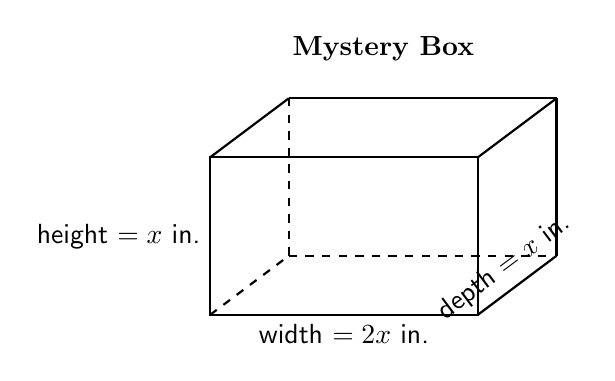
\begin{tikzpicture}[font=\sffamily]
  \def\w{3.4}
  \def\h{2.0}
  \coordinate (dx) at (1.0,0.75);

  \coordinate (fbl) at (0,0);
  \coordinate (fbr) at (\w,0);
  \coordinate (ftr) at (\w,\h);
  \coordinate (ftl) at (0,\h);
  \coordinate (bbl) at ($(fbl)+(dx)$);
  \coordinate (bbr) at ($(fbr)+(dx)$);
  \coordinate (btr) at ($(ftr)+(dx)$);
  \coordinate (btl) at ($(ftl)+(dx)$);

  % front face
  \draw[thick] (fbl) -- (fbr) -- (ftr) -- (ftl) -- cycle;
  % back-face hidden edges
  \draw[thick, dashed] (bbl) -- (bbr);
  \draw[thick, dashed] (bbl) -- (btl);
  % back-face visible edges
  \draw[thick] (bbr) -- (btr);
  \draw[thick] (btl) -- (btr);
  % connecting edges
  \draw[thick, dashed] (fbl) -- (bbl);
  \draw[thick] (fbr) -- (bbr);
  \draw[thick] (ftl) -- (btl);
  \draw[thick] (ftr) -- (btr);

  % title
  \node[font=\bfseries] at ($(ftl)!0.5!(btr)+(0,1.0)$) {Mystery Box};

  % dimension labels
  \node[below] at ($(fbl)!0.5!(fbr)$) {width $=2x$ in.};
  \node[left] at ($(fbl)!0.5!(ftl)$) {height $=x$ in.};
  \path (fbr) -- (bbr) node[midway, sloped, above] {depth $=x$ in.};
\end{tikzpicture}
\end{document}
